\newif\ifsolutions
\solutionstrue % Show solutions
%\solutionsfalse % Hide solutions

\documentclass{article}
\usepackage{geometry}
\geometry{margin=1in}
\usepackage{tikz}
\usepackage{amssymb}

% fleqn allows setting indent of display math
\usepackage[fleqn]{amsmath}
\setlength{\mathindent}{0pt} % Set indent
% Disable equation numbering (https://tex.stackexchange.com/a/360378)
\makeatletter
\renewcommand\tagform@[1]{}
\makeatother

% Allow Unicode (some, e.g., © and £ at least)
% https://tex.stackexchange.com/questions/370278/is-there-any-reason-to-use-inputenc
\usepackage[utf8]{inputenc}

% Hyperlinks
\usepackage{hyperref}
\hypersetup{colorlinks=true, urlcolor=blue, linkcolor=blue}

% Prevent indentation of paragraphs
\setlength\parindent{0pt}
\setlength{\parskip}{\baselineskip}

% Spacing above/below equations
% https://tex.stackexchange.com/a/69678
\AtBeginDocument{%
 \abovedisplayskip=-\parskip
 \abovedisplayshortskip=-\parskip
 \belowdisplayskip=0pt
 \belowdisplayshortskip=0pt
}

% Allow 3 additional subsection levels
% https://tex.stackexchange.com/a/60212
\usepackage{titlesec}
\setcounter{secnumdepth}{6}
% H4 in HTML
\titleformat{\paragraph}{\normalfont\normalsize\bfseries}{\theparagraph}{1em}{}
\titlespacing*{\paragraph}{0pt}{3.25ex plus 1ex minus .2ex}{1.5ex plus .2ex}
% H5 in HTML
\titleformat{\subparagraph}{\normalfont\normalsize\bfseries}{\thesubparagraph}{1em}{}
\titlespacing*{\subparagraph}{0pt}{3.25ex plus 1ex minus .2ex}{1.5ex plus .2ex}
% H6 in HTML
\titleformat{\subsubparagraph}{\normalfont\normalsize\bfseries}{\thesubsubparagraph}{1em}{}
\titlespacing*{\subsubparagraph}{0pt}{3.25ex plus 1ex minus .2ex}{1.5ex plus .2ex}

% So enumerate at all levels is numbers
% https://tex.stackexchange.com/questions/78842/nested-enumeration-numbering
\renewcommand{\labelenumii}{\arabic{enumii}.}
\renewcommand{\labelenumiii}{\arabic{enumiii}.}
\renewcommand{\labelenumiv}{\arabic{enumiv}.}

\renewcommand{\mbox}{\text}
\newcommand{\ds}[0]{\displaystyle}
\newcommand{\ihat}[0]{\hat{\boldsymbol{\imath}}}
\newcommand{\jhat}[0]{\hat{\boldsymbol{\jmath}}}
\newcommand{\khat}[0]{\hat{\boldsymbol{k}}}
\newcommand{\xhat}[0]{\hat{\mathbf{x}}}
\newcommand{\yhat}[0]{\hat{\mathbf{y}}}
\newcommand{\zhat}[0]{\hat{\mathbf{z}}}
\newcommand{\rhat}[0]{\hat{\mathbf{r}}}
\newcommand{\bfvec}[1]{\vec{\mathbf{#1}}}
\newcommand{\bfcdot}[0]{\boldsymbol{\cdot}}

\usepackage{fancyhdr}
\pagestyle{fancy}
\lhead{Kirchoff's Circuit Laws}
\rhead{\thepage}
\fancyfoot{}

\begin{document}

\section{Introduction}

To find the current through each resistor in a circuit with only batteries and resistors, Kirchhoff's Current Law and Kirchhoff's Voltage Rule can be used.

\begin{enumerate}

  \item Kirchhoff's Voltage Law (KVL): The sum of all voltage changes around a closed loop must equal zero.

  \item Kirchhoff's Current Law (KCL): The sum of all currents entering and exiting a junction must equal zero.

\end{enumerate}

\textbf{General procedure}

\begin{enumerate}

  \item Assume directions of current.

  \item Write equations for KCL for nodes.

  \item Write equations for KVL for loops using the assumed direction of current.

  \item Solve for currents.

\end{enumerate}

\textbf{Sign conventions}

If you get a negative number for a current, your assumed direction was wrong.

When you write KVL, you must choose a direction that you move around the loop. If you ``step" across a resistor $R$ in the direction of an assumed current $i$, the voltage change is $-iR$. If you ``step" across in the direction opposite of $i$, the voltage change is $iR$.

If you step across a battery with emf $\mathcal{E}$ from the $-$ to the $+$, the voltage change is $+\mathcal{E}$. If you step across a battery with emf $\mathcal{E}$ from the $+$ to the $-$, the voltage change is $-\mathcal{E}$. \emph{The direction of the assumed current does not matter.}

\newpage

\section{Single Loop Circuit}

In a single loop circuit, only KVL is needed to find the current.



\tikzset{every picture/.style={line width=0.75pt}} %set default line width to 0.75pt        

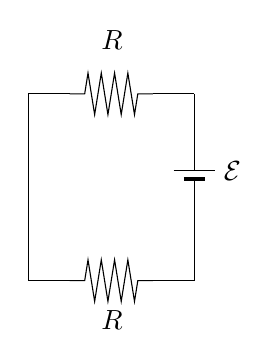
\begin{tikzpicture}[x=0.75pt,y=0.75pt,yscale=-1,xscale=1]
%uncomment if require: \path (0,165); %set diagram left start at 0, and has height of 165

%Shape: Resistor [id:dp04378564218643377] 
\draw   (33,39) -- (40.2,39) -- (41.8,29) -- (45,49) -- (48.2,29) -- (51.4,49) -- (54.6,29) -- (57.8,49) -- (61,29) -- (64.2,49) -- (65.8,39) -- (73,39) ;
%Straight Lines [id:da992166199236981] 
\draw    (73,39) -- (93,39) ;
%Straight Lines [id:da271365249390056] 
\draw    (93,39) -- (93,76) ;
%Straight Lines [id:da4991644356919813] 
\draw    (93,99) -- (93,129) ;
%Shape: Resistor [id:dp19059455882938692] 
\draw   (33,129) -- (40.2,129) -- (41.8,119) -- (45,139) -- (48.2,119) -- (51.4,139) -- (54.6,119) -- (57.8,139) -- (61,119) -- (64.2,139) -- (65.8,129) -- (73,129) ;
%Straight Lines [id:da5142725466949509] 
\draw    (73,129) -- (93,129) ;
%Straight Lines [id:da04358586309123358] 
\draw    (13,39) -- (33,39) ;
%Straight Lines [id:da17475123899038092] 
\draw    (13,129) -- (33,129) ;
%Straight Lines [id:da31864553225543846] 
\draw    (13,39) -- (13,129) ;
%Straight Lines [id:da23922847632173405] 
\draw    (83,76) -- (103,76) ;
%Straight Lines [id:da3747834408087263] 
\draw [line width=1.5]    (88,80) -- (98,80) ;
%Straight Lines [id:da9200807256957335] 
\draw    (93,80) -- (93,99) ;

% Text Node
\draw (47,7.4) node [anchor=north west][inner sep=0.75pt]    {$R$};
% Text Node
\draw (47,142.4) node [anchor=north west][inner sep=0.75pt]    {$R$};
% Text Node
\draw (106,70.4) node [anchor=north west][inner sep=0.75pt]    {$\mathcal{E}$};


\end{tikzpicture}


\begin{enumerate}

  \item Assume the direction of current $I$ in the above circuit is counterclockwise. Write the equation for KVL and then solve for $I$.

  \item Assume the direction of current $I$ in the following circuit is clockwise. Write the equation for KVL and then solve for $I$.

  \item Which value for $I$ found above is correct?

  \item If you removed the bottom resistor and replaced the top resistor with a resistor with resistance $2R$, would $I$ change?

\end{enumerate}

\section{Multiple Loop Circuit I}

Assume the direction of currents $I_1$, $I_2$, and $I_3$ in the following circuit are as shown.



\tikzset{every picture/.style={line width=0.75pt}} %set default line width to 0.75pt        

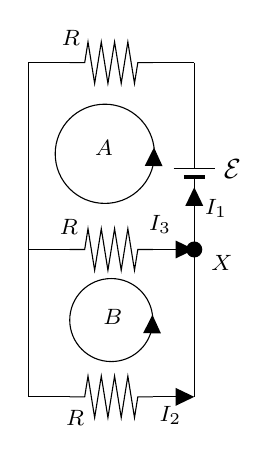
\begin{tikzpicture}[x=0.75pt,y=0.75pt,yscale=-1,xscale=1]
%uncomment if require: \path (0,212); %set diagram left start at 0, and has height of 212

%Shape: Resistor [id:dp4435768995868634] 
\draw   (33,20) -- (40.2,20) -- (41.8,10) -- (45,30) -- (48.2,10) -- (51.4,30) -- (54.6,10) -- (57.8,30) -- (61,10) -- (64.2,30) -- (65.8,20) -- (73,20) ;
%Straight Lines [id:da6348738339014448] 
\draw    (73,20) -- (93,20) ;
%Straight Lines [id:da5094119689345933] 
\draw    (93,20) -- (93,40) ;
%Straight Lines [id:da29132347297122374] 
\draw    (93,83) -- (93,110) ;
\draw [shift={(93,80)}, rotate = 90] [fill={rgb, 255:red, 0; green, 0; blue, 0 }  ][line width=0.08]  [draw opacity=0] (8.93,-4.29) -- (0,0) -- (8.93,4.29) -- cycle    ;
%Shape: Resistor [id:dp4960144413750487] 
\draw   (33,110) -- (40.2,110) -- (41.8,100) -- (45,120) -- (48.2,100) -- (51.4,120) -- (54.6,100) -- (57.8,120) -- (61,100) -- (64.2,120) -- (65.8,110) -- (73,110) ;
%Straight Lines [id:da24469614531440342] 
\draw    (73,110) -- (90,110) ;
\draw [shift={(93,110)}, rotate = 180] [fill={rgb, 255:red, 0; green, 0; blue, 0 }  ][line width=0.08]  [draw opacity=0] (8.93,-4.29) -- (0,0) -- (8.93,4.29) -- cycle    ;
%Straight Lines [id:da22765892469283] 
\draw    (13,20) -- (33,20) ;
%Straight Lines [id:da17732812907855178] 
\draw    (13,110) -- (33,110) ;
%Straight Lines [id:da9666768486239514] 
\draw    (13,20) -- (13,110) ;
%Shape: Resistor [id:dp6772651137474663] 
\draw   (33,181) -- (40.2,181) -- (41.8,171) -- (45,191) -- (48.2,171) -- (51.4,191) -- (54.6,171) -- (57.8,191) -- (61,171) -- (64.2,191) -- (65.8,181) -- (73,181) ;
%Straight Lines [id:da9288559665794871] 
\draw    (13,110) -- (13,181) ;
%Straight Lines [id:da06047002217821351] 
\draw    (93,110) -- (93,181) ;
\draw [shift={(93,110)}, rotate = 90] [color={rgb, 255:red, 0; green, 0; blue, 0 }  ][fill={rgb, 255:red, 0; green, 0; blue, 0 }  ][line width=0.75]      (0, 0) circle [x radius= 3.35, y radius= 3.35]   ;
%Straight Lines [id:da0286509869159568] 
\draw    (73,181) -- (90,181) ;
\draw [shift={(93,181)}, rotate = 180] [fill={rgb, 255:red, 0; green, 0; blue, 0 }  ][line width=0.08]  [draw opacity=0] (8.93,-4.29) -- (0,0) -- (8.93,4.29) -- cycle    ;
%Straight Lines [id:da6480632637542392] 
\draw    (13,181) -- (33,181) ;
%Shape: Arc [id:dp3431106756408584] 
\draw  [draw opacity=0] (73.47,67.89) .. controls (71.57,79.19) and (61.74,87.8) .. (49.9,87.8) .. controls (36.7,87.8) and (26,77.1) .. (26,63.9) .. controls (26,50.7) and (36.7,40) .. (49.9,40) .. controls (62.73,40) and (73.21,50.12) .. (73.78,62.81) -- (49.9,63.9) -- cycle ; \draw   (73.47,67.89) .. controls (71.57,79.19) and (61.74,87.8) .. (49.9,87.8) .. controls (36.7,87.8) and (26,77.1) .. (26,63.9) .. controls (26,50.7) and (36.7,40) .. (49.9,40) .. controls (62.73,40) and (73.21,50.12) .. (73.78,62.81) ;  
%Straight Lines [id:da24655244368311546] 
\draw    (73.47,67.89) -- (73.55,63.85) ;
\draw [shift={(73.61,60.85)}, rotate = 91.13] [fill={rgb, 255:red, 0; green, 0; blue, 0 }  ][line width=0.08]  [draw opacity=0] (8.93,-4.29) -- (0,0) -- (8.93,4.29) -- cycle    ;
%Shape: Arc [id:dp8851152110706482] 
\draw  [draw opacity=0] (72.72,147.34) .. controls (71.14,156.79) and (62.91,164) .. (53,164) .. controls (41.95,164) and (33,155.05) .. (33,144) .. controls (33,132.95) and (41.95,124) .. (53,124) .. controls (63.74,124) and (72.5,132.46) .. (72.98,143.09) -- (53,144) -- cycle ; \draw   (72.72,147.34) .. controls (71.14,156.79) and (62.91,164) .. (53,164) .. controls (41.95,164) and (33,155.05) .. (33,144) .. controls (33,132.95) and (41.95,124) .. (53,124) .. controls (63.74,124) and (72.5,132.46) .. (72.98,143.09) ;  
%Straight Lines [id:da6299489125610516] 
\draw    (72.72,147.34) -- (72.78,144.45) ;
\draw [shift={(72.84,141.45)}, rotate = 91.13] [fill={rgb, 255:red, 0; green, 0; blue, 0 }  ][line width=0.08]  [draw opacity=0] (8.93,-4.29) -- (0,0) -- (8.93,4.29) -- cycle    ;
%Straight Lines [id:da035127828787047566] 
\draw    (93,34) -- (93,71) ;
%Straight Lines [id:da06981066985977469] 
\draw    (83,71) -- (103,71) ;
%Straight Lines [id:da07498872749287244] 
\draw [line width=1.5]    (88,75) -- (98,75) ;
%Straight Lines [id:da9169274458375447] 
\draw    (93,75) -- (93,94) ;

% Text Node
\draw (27,94.4) node [anchor=north west][inner sep=0.75pt]  [font=\footnotesize]  {$R$};
% Text Node
\draw (97,84.4) node [anchor=north west][inner sep=0.75pt]  [font=\footnotesize]  {$I_{1}$};
% Text Node
\draw (75,184.4) node [anchor=north west][inner sep=0.75pt]  [font=\footnotesize]  {$I_{2}$};
% Text Node
\draw (70,92.4) node [anchor=north west][inner sep=0.75pt]  [font=\footnotesize]  {$I_{3}$};
% Text Node
\draw (100,111.4) node [anchor=north west][inner sep=0.75pt]  [font=\footnotesize]  {$X$};
% Text Node
\draw (44,56.4) node [anchor=north west][inner sep=0.75pt]  [font=\footnotesize]  {$A$};
% Text Node
\draw (30,186.4) node [anchor=north west][inner sep=0.75pt]  [font=\footnotesize]  {$R$};
% Text Node
\draw (28,3.4) node [anchor=north west][inner sep=0.75pt]  [font=\footnotesize]  {$R$};
% Text Node
\draw (48,137.4) node [anchor=north west][inner sep=0.75pt]  [font=\footnotesize]  {$B$};
% Text Node
\draw (106,65.4) node [anchor=north west][inner sep=0.75pt]    {$\mathcal{E}$};


\end{tikzpicture}


\begin{enumerate}

  \item Write the equation for KVL for loop A.

  \item Write the equation for KVL for loop B.

  \item Write the equation for KCL for node X.

\end{enumerate}

Use the three equations found above to solve for the three unknowns, $I_1$, $I_2$, and $I_3$.

\newpage

\section{Multiple Loop Circuit II}

In the circuit for the previous problem, there are three possible loops. The third loop is loop C. indicated below.



\tikzset{every picture/.style={line width=0.75pt}} %set default line width to 0.75pt        

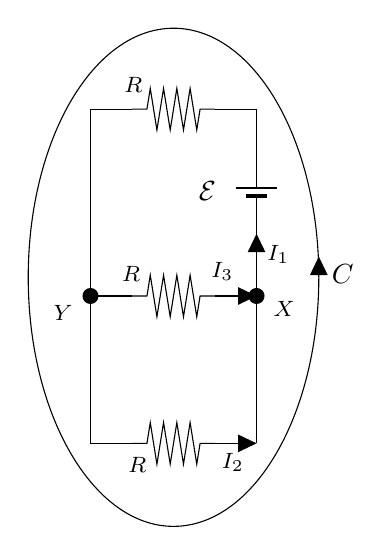
\begin{tikzpicture}[x=0.75pt,y=0.75pt,yscale=-1,xscale=1]
%uncomment if require: \path (0,264); %set diagram left start at 0, and has height of 264

%Shape: Resistor [id:dp17060205471087664] 
\draw   (60,49) -- (67.2,49) -- (68.8,39) -- (72,59) -- (75.2,39) -- (78.4,59) -- (81.6,39) -- (84.8,59) -- (88,39) -- (91.2,59) -- (92.8,49) -- (100,49) ;
%Straight Lines [id:da026559281912648114] 
\draw    (100,49) -- (120,49) ;
%Straight Lines [id:da7617206491414388] 
\draw    (120,49) -- (120,69) ;
%Straight Lines [id:da970382599927843] 
\draw    (120,112) -- (120,139) ;
\draw [shift={(120,109)}, rotate = 90] [fill={rgb, 255:red, 0; green, 0; blue, 0 }  ][line width=0.08]  [draw opacity=0] (8.93,-4.29) -- (0,0) -- (8.93,4.29) -- cycle    ;
%Shape: Resistor [id:dp606783941498729] 
\draw   (60,139) -- (67.2,139) -- (68.8,129) -- (72,149) -- (75.2,129) -- (78.4,149) -- (81.6,129) -- (84.8,149) -- (88,129) -- (91.2,149) -- (92.8,139) -- (100,139) ;
%Straight Lines [id:da17314151648314247] 
\draw    (100,139) -- (117,139) ;
\draw [shift={(120,139)}, rotate = 180] [fill={rgb, 255:red, 0; green, 0; blue, 0 }  ][line width=0.08]  [draw opacity=0] (8.93,-4.29) -- (0,0) -- (8.93,4.29) -- cycle    ;
%Straight Lines [id:da8025234315851337] 
\draw    (40,49) -- (60,49) ;
%Straight Lines [id:da17836496817482805] 
\draw    (40,139) -- (60,139) ;
%Straight Lines [id:da7781781144106024] 
\draw    (40,49) -- (40,139) ;
%Shape: Resistor [id:dp2826362414149479] 
\draw   (60,210) -- (67.2,210) -- (68.8,200) -- (72,220) -- (75.2,200) -- (78.4,220) -- (81.6,200) -- (84.8,220) -- (88,200) -- (91.2,220) -- (92.8,210) -- (100,210) ;
%Straight Lines [id:da8251219225767277] 
\draw    (120,139) -- (120,210) ;
\draw [shift={(120,139)}, rotate = 90] [color={rgb, 255:red, 0; green, 0; blue, 0 }  ][fill={rgb, 255:red, 0; green, 0; blue, 0 }  ][line width=0.75]      (0, 0) circle [x radius= 3.35, y radius= 3.35]   ;
%Straight Lines [id:da4634026204005979] 
\draw    (100,210) -- (117,210) ;
\draw [shift={(120,210)}, rotate = 180] [fill={rgb, 255:red, 0; green, 0; blue, 0 }  ][line width=0.08]  [draw opacity=0] (8.93,-4.29) -- (0,0) -- (8.93,4.29) -- cycle    ;
%Straight Lines [id:da022515967651009827] 
\draw    (40,210) -- (60,210) ;
%Shape: Ellipse [id:dp5645644533895287] 
\draw   (10,130) .. controls (10,63.73) and (41.34,10) .. (80,10) .. controls (118.66,10) and (150,63.73) .. (150,130) .. controls (150,196.27) and (118.66,250) .. (80,250) .. controls (41.34,250) and (10,196.27) .. (10,130) -- cycle ;
%Straight Lines [id:da018587299401993995] 
\draw    (150,130) -- (150,123) ;
\draw [shift={(150,120)}, rotate = 90] [fill={rgb, 255:red, 0; green, 0; blue, 0 }  ][line width=0.08]  [draw opacity=0] (8.93,-4.29) -- (0,0) -- (8.93,4.29) -- cycle    ;
%Straight Lines [id:da8059012117058191] 
\draw    (40,139) -- (40,210) ;
\draw [shift={(40,139)}, rotate = 90] [color={rgb, 255:red, 0; green, 0; blue, 0 }  ][fill={rgb, 255:red, 0; green, 0; blue, 0 }  ][line width=0.75]      (0, 0) circle [x radius= 3.35, y radius= 3.35]   ;
%Straight Lines [id:da9608319101186609] 
\draw    (120,50) -- (120,87) ;
%Straight Lines [id:da022039084729565506] 
\draw    (110,87) -- (130,87) ;
%Straight Lines [id:da0036845135841885313] 
\draw [line width=1.5]    (115,91) -- (125,91) ;
%Straight Lines [id:da22758616610747429] 
\draw    (120,91) -- (120,110) ;

% Text Node
\draw (54,123.4) node [anchor=north west][inner sep=0.75pt]  [font=\footnotesize]  {$R$};
% Text Node
\draw (124,113.4) node [anchor=north west][inner sep=0.75pt]  [font=\footnotesize]  {$I_{1}$};
% Text Node
\draw (102,213.4) node [anchor=north west][inner sep=0.75pt]  [font=\footnotesize]  {$I_{2}$};
% Text Node
\draw (97,121.4) node [anchor=north west][inner sep=0.75pt]  [font=\footnotesize]  {$I_{3}$};
% Text Node
\draw (127,140.4) node [anchor=north west][inner sep=0.75pt]  [font=\footnotesize]  {$X$};
% Text Node
\draw (57,215.4) node [anchor=north west][inner sep=0.75pt]  [font=\footnotesize]  {$R$};
% Text Node
\draw (55,32.4) node [anchor=north west][inner sep=0.75pt]  [font=\footnotesize]  {$R$};
% Text Node
\draw (155,122.4) node [anchor=north west][inner sep=0.75pt]    {$C$};
% Text Node
\draw (21,142.4) node [anchor=north west][inner sep=0.75pt]  [font=\footnotesize]  {$Y$};
% Text Node
\draw (91,82.4) node [anchor=north west][inner sep=0.75pt]    {$\mathcal{E}$};


\end{tikzpicture}


\begin{enumerate}

  \item Write the equation for KVL for loop C.

  \item Use the equation for KVL for loop B. and the KCL equation for node X from the previous problem along with the KVL equation for loop C to find $I_1$, $I_2$, and $I_3$. (You should get the same answers.)

\end{enumerate}

\section{Redundant Equations}

When solving circuit problems with multiple loops, you will generally find that you can use KVL and KCL to write more equations than there are unknowns. If you encounter a situation where you wrote $N$ equations based on KVL and KCL but cannot find $N$ unknows, the reason is that two or more of the $N$ equations that you wrote were not independent. To demonstrate this, for the circuit below,

\begin{enumerate}

  \item Write the KCL equation for node X

  \item Write the KCL equation for node Y

  \item Write the KVL equation for loop A

  \item Attempt to use the above three equations to solve for $I_1$, $I_2$, and $I_3$.

\end{enumerate}

\end{document}